\subsection{Enfoque}

\subsection{Enfoque}

Este proyecto se ha organizado en cuatro fases principales, cada una de las cuales está alineada con las asignaturas del máster en Ciencia de Datos y Big Data. A continuación se detallan las fases y las asignaturas involucradas en cada una:
\begin{figure}[H]
    \centering
    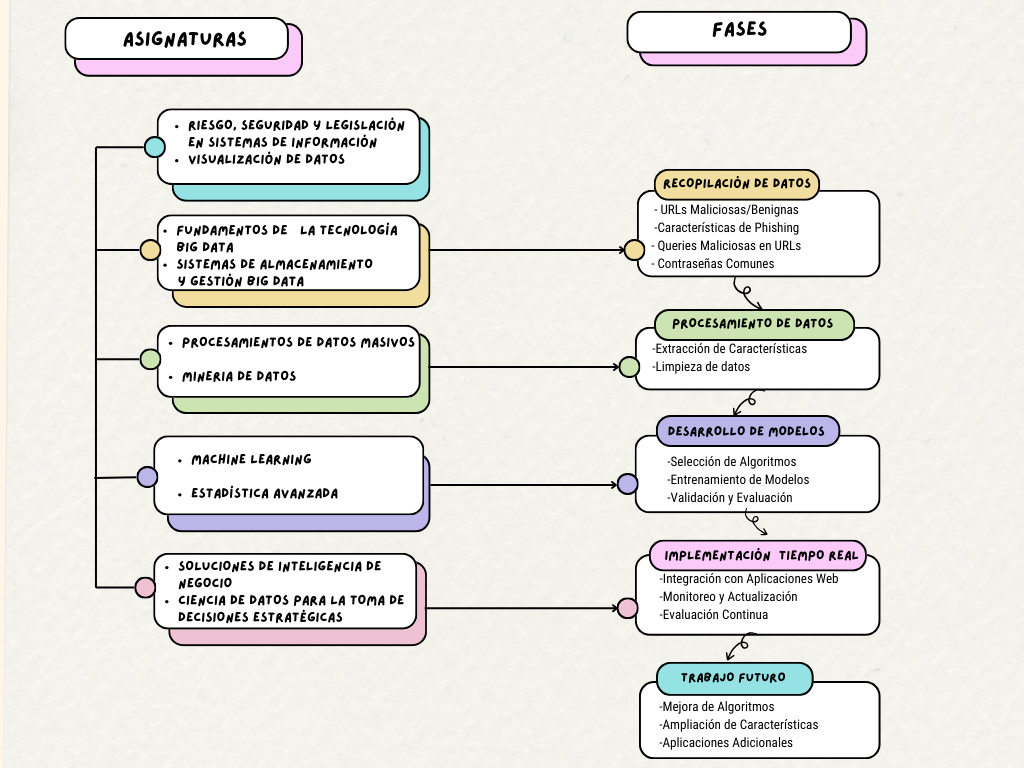
\includegraphics[width=0.8\textwidth]{imagenn1.png}
    \caption{Fases del Proyecto y Asignaturas del Máster}
\end{figure}
\begin{enumerate}
    \item \textbf{Recopilación de Datos}: 
    \begin{itemize}
        \item Asignaturas: Fundamentos de la Tecnología Big Data, Sistemas de Almacenamiento y Gestión Big Data.
        \item Actividades: Recolección de URLs maliciosas y benignas, características de phishing, queries maliciosas en URLs y contraseñas comunes.
    \end{itemize}

    \item \textbf{Procesamiento de Datos}:
    \begin{itemize}
        \item Asignaturas: Procesamientos de Datos Masivos, Minería de Datos.
        \item Actividades: Extracción de características y limpieza de datos.
    \end{itemize}

    \item \textbf{Desarrollo de Modelos}:
    \begin{itemize}
        \item Asignaturas: Machine Learning, Estadística Avanzada.
        \item Actividades: Selección de algoritmos, entrenamiento de modelos, validación y evaluación.
    \end{itemize}

    \item \textbf{Implementación en Tiempo Real}:
    \begin{itemize}
        \item Asignaturas: Soluciones de Inteligencia de Negocio, Ciencia de Datos para la Toma de Decisiones Estratégicas.
        \item Actividades: Integración con aplicaciones web, monitoreo y actualización, evaluación continua.
    \end{itemize}
\end{enumerate}

El sistema desarrollado consta de varios componentes clave, como se ilustra en las figuras a continuacion. A continuación se describe el flujo del sistema:
\begin{figure}[H]
    \centering
    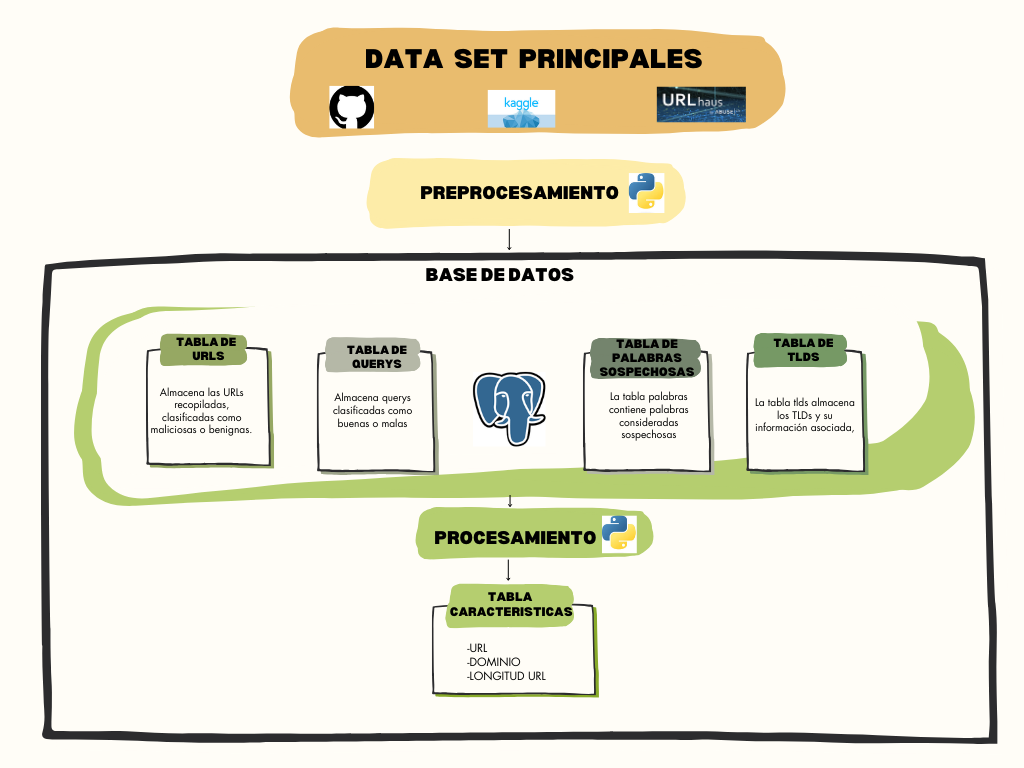
\includegraphics[width=0.8\textwidth]{imagenn2.png}
    \caption{Arquitectura del Sistema: Dataset, Preprocesamiento y Base de Datos}
\end{figure}

\begin{figure}[H]
    \centering
    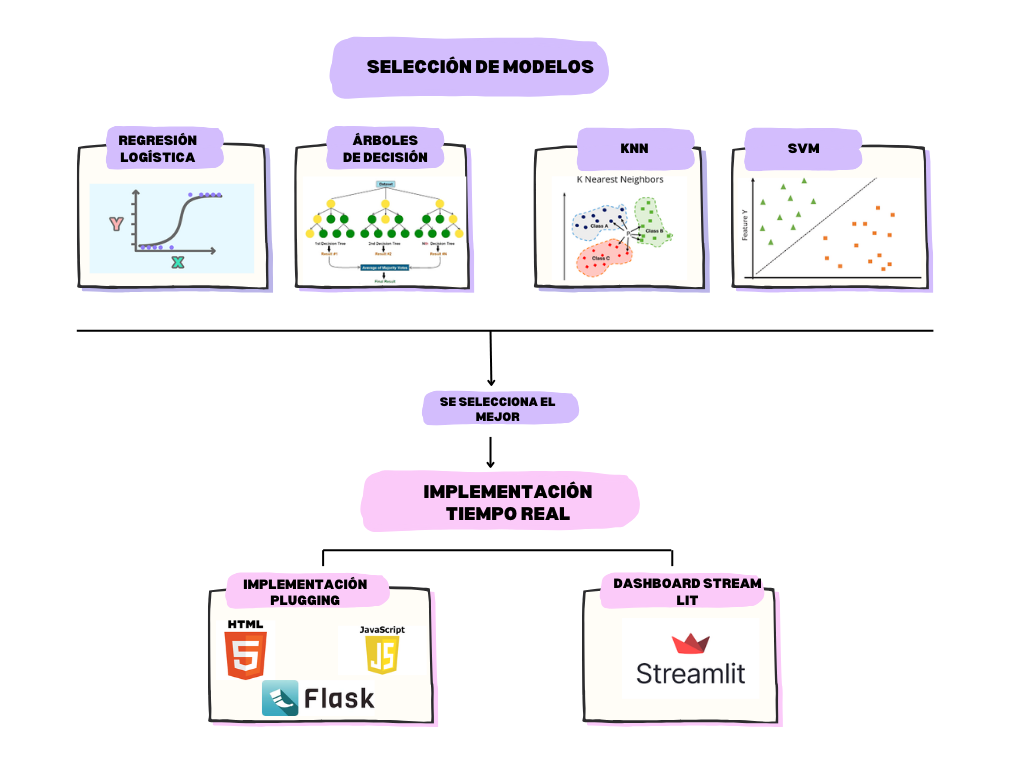
\includegraphics[width=0.8\textwidth]{imagenn3.png}
    \caption{Selección de Modelos e Implementación en Tiempo Real}
\end{figure}

\begin{itemize}
    \item \textbf{Dataset Principal y Preprocesamiento}: 
    Los datos recopilados de fuentes como Kaggle, GitHub y URLhaus son preprocesados usando Python y almacenados en una base de datos estructurada (Figura 2).
    
    \item \textbf{Base de Datos y Tablas de Características}: 
    La base de datos contiene tablas para almacenar URLs, queries, palabras sospechosas y TLDs. Las características extraídas de las URLs se almacenan en una tabla específica de características (Figura 2).
    
    \item \textbf{Selección y Entrenamiento de Modelos}: 
    Se evaluaron varios algoritmos de machine learning, incluyendo regresión logística, árboles de decisión, KNN y SVM, para seleccionar el mejor modelo para la detección de URLs maliciosas (Figura 3).
    
    \item \textbf{Implementación en Tiempo Real}: 
    El modelo seleccionado se implementó en un plugin usando HTML, JavaScript y Flask, y se desarrolló un dashboard interactivo con Streamlit para la visualización y análisis de datos (Figura 3).
\end{itemize}

Las herramientas utilizadas en este proyecto incluyen Python para el procesamiento de datos y desarrollo de modelos, Google Documents y GitHub para la documentación y gestión de versiones, Trello para la gestión del proyecto, Visual Studio para el desarrollo de código, Overleaf para la escritura de LaTeX, PowerPoint para las presentaciones, y Streamlit para el desarrollo del dashboard.



